\documentclass[a4paper,11pt]{report}

%%%%%%%%%%%%
% packages %
%%%%%%%%%%%%
\usepackage{caption}
\usepackage{color}
\usepackage[english]{babel}
\usepackage[utf8x]{inputenc}
\usepackage{lmodern}
\usepackage[T1]{fontenc}

\usepackage{listings}
\usepackage{microtype}
\usepackage{avant}

\usepackage{graphicx}
\usepackage{fancyhdr}
\usepackage{pgfgantt}

%% Maths symbols
\usepackage{amsmath}
\usepackage{amssymb}

% float figures forcing
\usepackage{placeins}
% GNUPLOT
%\usepackage{gnuplot-lua-tikz}

\usepackage{sectsty}

%%%%%%%%%%%%%%%%%%%
% custom commands %
%%%%%%%%%%%%%%%%%%%
\newcommand{\HRule}{\rule{\linewidth}{0.5mm}}
%\usepackage[left=3cm,right=3cm,top=2cm,bottom=2cm]{geometry}
\usepackage{geometry}


%%%%%%%%%%%%%%
% new colors %
%%%%%%%%%%%%%%
% solarized colors
\definecolor{base03}{HTML}{002B36}
\definecolor{base02}{HTML}{073642}
\definecolor{base01}{HTML}{586E75}
\definecolor{base00}{HTML}{657B83}
\definecolor{base0}{HTML}{839496}
\definecolor{base1}{HTML}{93A1A1}
\definecolor{base2}{HTML}{EEE8D5}
\definecolor{base3}{HTML}{FDF6E3}
\definecolor{yellow}{HTML}{B58900}
\definecolor{orange}{HTML}{CB4B16}
\definecolor{red}{HTML}{DC322F}
\definecolor{magenta}{HTML}{D33682}
\definecolor{violet}{HTML}{6C71C4}
\definecolor{blue}{HTML}{268BD2}
\definecolor{cyan}{HTML}{2AA198}
\definecolor{green}{HTML}{859900}

\definecolor{defaultFontColor}{HTML}{073642} % base 02

%%%%%%%%%
% fonts %
%%%%%%%%%
% inconsolata %
\usepackage{inconsolata}
%\renewcommand*\familydefault{\ttdefault} %% Only if the base font of the document is to be typewriter style
%\usepackage[T1]{fontenc}
\renewcommand*\familydefault{\rmdefault}\color{defaultFontColor} %% Only if the base font of the document is to be typewriter style

\chapterfont{\color{red}}
\sectionfont{\color{orange}}
\subsectionfont{\color{blue}}
\paragraphfont{\color{base01}}
\paragraphfont{\color{base2}}
\subparagraphfont{\color{base2}}

% title specific %
% title rule
\newcommand{\titleRule}{\color{base2}\HRule\color{defaultFontColor}}

%%%%%%%%%%%%%%%%%%%%
% listing settings %
%%%%%%%%%%%%%%%%%%%%
\lstset{
    basicstyle=\ttfamily\small,
    language=bash,
    frame=lines,
    sensitive=true
    tabsize=2,
    breaklines=true,
    showstringspaces=false,
    showspaces=false,
    backgroundcolor=\color{base3},
    keywordstyle=\color{blue},
    commentstyle=\color{base1},
    stringstyle=\color{cyan},
    numberstyle=\color{violet},
    rulecolor=\color{base00},
    morekeywords={pfw, setParameter, getParameter}
}

%%%%%%%%%%%%%%%%%%%%
% caption settings %
%%%%%%%%%%%%%%%%%%%%
\DeclareCaptionFont{captionText}{\color{base1}}
\DeclareCaptionFormat{listing}{\colorbox{base03}{\parbox{0.985\textwidth}{\hspace{15pt}#1#2#3}}}
\captionsetup[lstlisting]{format=listing,labelfont=captionText,textfont=captionText, singlelinecheck=true, margin=0pt, font={sf,footnotesize}}
\DeclareCaptionFormat{figure}{\colorbox{base03}{\parbox{0.985\textwidth}{\hspace{15pt}#1#2#3}}}
\captionsetup[figure]{format=figure,labelfont=captionText,textfont=captionText, singlelinecheck=false, margin=0pt, font={sf,footnotesize}}

%%%%%%%%%%%%%%%%%%%%%%
% pagestyle settings %
%%%%%%%%%%%%%%%%%%%%%%
\pagestyle{fancy}
\renewcommand{\headrulewidth}{0.4pt}
\fancyhead{}
\fancyhead[LE]{\textit{\nouppercase{\leftmark}}}
\fancyhead[RO]{\textit{\nouppercase{\rightmark}}}
\fancyfoot{}
\fancyfoot[C]{\thepage}

\usepackage{hyperref}
% Hyperref setup
\hypersetup{colorlinks=true}
\hypersetup{urlcolor=blue}
\hypersetup{citecolor=dkgreen}


% make use of glossary
\usepackage{glossaries}
\makeglossaries
% Thanks to Apelete Seketeli <apelete@seketeli.org> for this glossary.

% $0 glossary entries: UMG, MeeGo, Android, PSI, Medfield, MID, SoC

% define an acronym using \newglossaryentry
%\newglossaryentry{umg}
%{
% how the entry name should appear in the glossary
%  name=UMG (Ultra Mobility Group),
%% how the description should appear in the glossary
%  description={Intel's department responsible for focusing core
%    processor and chipset business on mobile platforms},
%% how the entry should appear in the document text
%  text=UMG,
%% how the entry should appear the first time it is used in the
%% document text
%
%  first=Ultra Mobility Group (UMG)
%}

\newglossaryentry{umg}
{
  name=UMG (Ultra Mobility Group),
  description={Intel's department responsible for focusing core
    processor and chipset business on mobile platforms},
  text=UMG,
  first=Ultra Mobility Group (UMG)
}

\newglossaryentry{meego}
{
  name=MeeGo\textsuperscript{\texttrademark},
  description={A Linux-based open source mobile operating system
    jointly created by Intel and Nokia}
}

\newglossaryentry{android}
{
  name=Android,
  description={Google's software stack for mobile devices, based on
  the Linux kernel, that includes an operating system, middleware and
  key applications}
}

\newglossaryentry{hal}
{
  name=HAL (Hardware Abstraction Layer),
  description={A set of routines that eases the access to a
  platform's hardware resources},
  text=HAL,
  first=Hardware Abstraction Layer (HAL)
}

\newglossaryentry{gerrit}
{
  name=Gerrit,
  description={Android's official web based code review system.
  It uses Git as version control system}
}

\newglossaryentry{vanilla}
{
  name=Vanilla (code base),
  description={Vanilla software is software which is not customized. It is in its original form.
  For example, vanilla Android is Android such as provided from Google, without any modifications},
  text=vanilla
}

\newglossaryentry{pfw}
{
  name=Parameter-framework,
  description={Intel audio team's generic solution to allow system-wide
  parameter management. It is configured via Structure and Settings files.
  It relies on an open plugin architecture to support systems such as audio,
  Bluetooth, Energy Management and more}
}

\newglossaryentry{scrum}
{
  name=Scrum,
  description={One of the most known implementation of Agile software development.
  It is a flexible, holistic product development strategy where a development team
  works as a unit to reach a common goal}
}

\newglossaryentry{markdown}
{
  name=Markdown,
  description={A plain-text based language which is used to quickly write documents.
  Those files can be converted into HTML, LaTex, PDF, or other formats.
  It is extremely popular for readme files}
}

\newglossaryentry{GitHub}
{
  name=GitHub,
  description={A web-based source-code repository hosting service based on Git.
  It is free for open-source projects and contains more than ten million repositories.
  Some big companies such as Adobe, and Microsoft have open-source components hosted on
  it}
}

\newglossaryentry{pullrequests}
{
  name=Pull requests,
  description={A standard way to contribute to git projects. Based on the fork \& pull model.
  See \url{https://help.github.com/articles/using-pull-requests} for more information}
}

\newglossaryentry{python}
{
  name=Python,
  description={A widely used multi-purpose language, with a huge standard library.
  It is mostly used for scripting tasks, but can be used for everything.
  Python was invented by Guido van Rossum, in Holland}
}

\newglossaryentry{cpp}
{
  name=C++,
  description={A multi-paradigm, powerful, compiled programming language. C++ is multi-purpose, even mostly used
  in scenarios where performance matters}
}

\newglossaryentry{aosp}
{
  name=AOSP (Android Open-Source Project),
  description={The Android Open-Source Project led by Google},
  text=AOSP,
  first=Android OpenSource Project (AOSP)
}

\newglossaryentry{alsa}
{
  name=ALSA (Advanced Linux Sound Architecture),
  description={Linux kernel component responsible of handling the Linux audio stack},
  text=ALSA,
  first=Advanced Linux Sound Architecture (ALSA)
}

\newglossaryentry{psi}
{
  name=PSI (Platform Software Integration),
  description={A division of UMG, responsible for the integration and
    validation of the software components for the future Intel mobile
    phone platform},
  text=PSI,
  first=Platform Software Integration (PSI)
}

\newglossaryentry{medfield}
{
  name=Medfield,
  description={Intel's fourth generation Mobile Internet Device
    platform. It is build around an Intel System-on-Chip which
    contains a 32nm Intel Atom\textsuperscript{\texttrademark}
    processor}
}

\newglossaryentry{mid}
{
  name=MID (Mobile Internet Device),
  description={A multimedia-capable mobile device providing wireless
    Internet access},
  text=MID,
  first=Mobile Internet Devices (MID)
}

\newglossaryentry{soc}
{
  name=SoC (System-on-Chip),
  description={Refers to integrating all components of a computer or
    other electronic system into a single integrated circuit},
  text=SoC,
  first=System-on-Chip (SoC)
}

% $1 glossary entries: Atom, ODM, OS, Autotools, Makefile, Logic
% analyzer, GDB, strace, Git, Kernel, Latex, Penwell, MSIC, 3G, iCDK,
% eMMC, kboot, Firmware

\newglossaryentry{atom}
{
  name=Intel Atom\textsuperscript{\texttrademark},
  description={The brand name for a line of ultra-low-voltage x86 and
    x86-64 microprocessors from Intel, used mainly in netbooks and
    Mobile Internet Devices},
  text=Atom,
  first=Intel Atom\textsuperscript{\texttrademark}
}
\newglossaryentry{xml}
{
  name=XML (Extensible Markup Language),
  description={A set of rules for encoding documents in
    machine-readable form. The design goals of XML emphasize
    simplicity, generality, and usability over the Internet. It is a
    textual data format with strong support via Unicode for the
    languages of the world. Although the design of XML focuses on
    documents, it is widely used for the representation of arbitrary
    data structures, for example in web services},
  text=XML,
  first=Extensible Markup Language (XML)
}

\newglossaryentry{xsd}
{
  name=XSD (XML Schema Definition),
  description={A format to formally describe XML elements. It can be
  used by developers to verify that the XML files respect certain constraints
  },
  text=XSD,
  first=XML Schema Definition (XSD)
}

\newglossaryentry{odm}
{
  name=ODM (Original Design Manufacturer),
  description={A company which designs and manufactures a product
    which is specified and eventually branded by another firm for
    sale},
  text=ODM,
  first=Original Design Manufacturers (ODM)
}

\newglossaryentry{msic}
{
  name=MSIC (Mixed Signal Integrated Circuit),
  description={Any integrated circuit that has both analog circuits
    and digital circuits on a single semiconductor die},
  text=MSIC,
  first=Mixed Signal Integrated Circuit (MSIC)
}

\newglossaryentry{os}
{
  name=OS (Operating System),
  description={A software that runs on computers, manages computer
    hardware resources, and provides common services for execution of
    various application software. Without an operating system, a user
    cannot run an application program on his computer, unless the
    application program is self booting},
  text=OS,
  first=Operating Systems (OS)
}

\newglossaryentry{autotools}
{
  name=Autotools,
  description={The GNU build system, also known as the Autotools, is a
    suite of programming tools designed to assist in making
    source-code packages portable to many Unix-like systems},
  text=autotools
}

\newglossaryentry{makefile}
{
  name=Makefile,
  description={In software development, ``make'' is a utility that
    automatically builds executable programs and libraries from source
    code, by reading files called makefiles which specify how to
    derive the target program},
  text=makefile
}

\newglossaryentry{logic analyzer}
{
  name=Logic Analyzer,
  description={An electronic instrument which displays signals in a
    digital circuit. For PC-based analyzers, the hardware connects to
    a computer through a USB or Ethernet connection and then relays
    the captured signals to the software on the computer},
  text=logic analyzer
}

\newglossaryentry{gdb}
{
  name=GDB (GNU Debugger),
  description={The GNU Debugger is the standard debugger for the GNU
    software system. It is a portable debugger that runs on many
    Unix-like systems and works for many programming languages},
  text=GDB,
  first=GNU Debugger (GDB)
}

\newglossaryentry{strace}
{
  name=Strace,
  description={A debugging utility in Linux to monitor the system
    calls used by a program and all the signals it receives},
  text=strace
}

\newglossaryentry{git}
{
  name=Git,
  description={A distributed revision control system with an emphasis
    on speed. Git was initially designed and developed by Linus
    Torvalds for Linux kernel development},
}

\newglossaryentry{vim}
{
  name=Vim,
  description={A modal text editor, based on vi, and maintained by Bram Moolenaar.
  Its power comes from its different modes, motions, and its extensibility}
}

\newglossaryentry{tmux}
{
  name=Tmux,
  description={The terminal multiplexer. Is very useful to organize multiple terminal instances in
  one terminal emulator. It handles splits, multiple pane layouts, and is fully configurable via a
  configuration file}
}

\newglossaryentry{kernel}
{
  name=Linux kernel,
  description={A set of components that translates software requests into data processing instructions
   for the underlying hardware. The Linux kernel is one of the most prominent
    examples of free and open source software},
  text=kernel
}

\newglossaryentry{latex}
{
  name=\LaTeX,
  description={A document markup language and document preparation
    system for the TeX typesetting program. The term LaTeX refers only
    to the language in which documents are written, not to the editor
    used to write those documents},
}

\newglossaryentry{penwell}
{
  name=Penwell,
  description={Le nom de code du system-on-Chip qui contient le notament le processeur
   central Atom},
  text=Penwell
}

\newglossaryentry{ifx}
{
  name=IFX (Infineon),
  description={The codename of the Infineon modem on the software
    development plateform. Infineon Technologies AG is a German
    semiconductor manufacturer and was founded in 1999, when the
    semiconductor operations of the parent company Siemens AG were
    spun off to form a separate legal entity},
  text=IFX,
  first=Infineon (IFX)
}

\newglossaryentry{3g}
{
  name=3G,
  description={Also known as ``3rd generation mobile
    telecommunications'', it is a generation of standards for mobile
    phones and mobile telecommunication services. Application services
    include wide-area wireless voice telephone, mobile Internet
    access, video calls and mobile TV, all in a mobile
    environment. Recent 3G releases, often denoted 3.5G and 3.75G,
    also provide mobile broadband access of several Mbit/s to
    smartphones and mobile modems in laptop computers}
}

\newglossaryentry{ti}
{
  name=TI (Texas Instrument),
  description={An American company founded in 1930, which develops and
    commercializes semiconductor and computer technology. Texas
    Instrument is one of the largest manufacturer of semiconductors
    worldwide after Intel},
  text=TI,
  first=Texas Instrument (TI)
}

\newglossaryentry{icdk}
{
  name=iCDK (Intel Customer Development Kit),
  description={The codename of the Intel software development
    platform. It is a printed circuit board containing an Intel
    System-on-Chip, electronic components and peripherals from various
    hardware manufacturers},
  text=iCDK,
  first=Intel Customer Development Kit (iCDK)
}

\newglossaryentry{emmc}
{
  name=eMMC (Embedded MultiMedia Card),
  description={A flash memory card standard. eMMC describes an
    architecture consisting of an embedded storage solution, flash
    memory and controller, all in a small package},
  text=eMMC
}

\newglossaryentry{kboot}
{
  name=Kboot,
  description={A proof-of-concept implementation of a Linux
    bootloader. This relatively small program is needed to access the
    nonvolatile devices from which the operating system programs and
    data are loaded},
  text=kboot
}

\newglossaryentry{firmware}
{
  name=Firmware,
  description={A fixed, usually rather small, program and/or data
    structure that internally control various electronic devices such
    as remote controls, calculators, hard disks, keyboards or memory
    cards},
  text=firmware
}

% $2 glossary entries: Pulseaudio, PCM, ACS, API, Driver, SSP, I2S,
% KTS

\newglossaryentry{pulseaudio}
{
  name=PulseAudio,
  description={A cross-platform, networked sound server commonly used
    on the Linux-based and FreeBSD operating systems. One of the goals
    of PulseAudio is to reroute all sound streams through it,
    including those from processes that attempt to directly access the
    hardware}
}

\newglossaryentry{pomodoro}
{
  name=Pomodoro technique,
  description={A time management technique which is frequently used by software developers.
  The technique uses a timer to break down work into intervals traditionally 25 minutes in length, separated by short breaks.
  The method is based on the idea that frequent breaks can improve mental agility
  },
  text=Pomodoro technique
}



\newglossaryentry{pcm}
{
  name=PCM (Pulse-Code Modulation),
  description={A method used to digitally represent sampled analog
    signals. It is the standard form for digital audio in computers as
    well as digital telephone systems},
  text=PCM,
  first=Pulse-Code Modulation (PCM)
}

\newglossaryentry{acs}
{
  name=ACS (Automation Control System),
  description={An automation and test sequencing tool developed by
    Intel. It is written in Python and serves test requirements at the
    middleware level. It was chosen as a solution to automate the
    audio quality checker tool},
  text=ACS,
  first=Automation Control System (ACS)
}

\newglossaryentry{api}
{
  name=API (Application Programming Interface),
  description={A particular set of rules (`code') and specifications
    that software programs can follow to communicate with each
    other. It serves as an interface between different software
    programs and facilitates their interaction},
  text=API,
  first=Application Programming Interface (API)
}

\newglossaryentry{driver}
{
  name=Device driver,
  description={A computer program allowing higher-level computer
    programs to interact with a hardware device},
  text=driver,
  first=device drivers
}

\newglossaryentry{ssp}
{
  name=SSP (Synchronous Serial Port),
  description={A controller that supports the Serial Peripheral
    Interface and Integrated Interchip Sound interface. It uses a
    master-slave paradigm to communicate across its connected bus},
  text=SSP,
  first=Synchronous Serial Port (SSP)
}


\newglossaryentry{kts}
{
  name=KTS (Kernel Test Suite),
  description={A suite of test programs for audio quality assurance at
    the driver level. The programs in this suite are aimed at the
    audio hardware devices in Medfield, but currently provide test
    routines for the bluetooth and modem chip},
  text=KTS,
  first=Kernel Test Suite (KTS)
}

% $3 glossary entries: LPE, DMAC, FIFO, MISO, MOSI, SPI, BlueZ, HCI,
% UART, IOCTL, ssploop, sspconf, AT commands, KGDB, dmesg, GPL, Free
% Software, Gitorious, XML

\newglossaryentry{lpe}
{
  name=LPE (Low Power Engine),
  description={A circuit of the Intel System-on-Chip responsible for
    audio processing. It is designed to process Pulse-Code Modulation
    data as well as compressed audio data while being power efficient},
  text=LPE,
  first=Low Power Engine (LPE)
}

\newglossaryentry{dmac}
{
  name=DMAC (Direct Memory Access Controller),
  description={A controller that allows certain hardware subsystems
    within the computer to access system memory for reading and/or
    writing independently of the central processing unit. Without
    Direct Memory Access, the central processing unit is typically
    fully occupied for the entire duration of the read or write
    operation, and is thus unavailable to perform other work. With
    Direct Memory Access, the central processing unit would initiate
    the transfer, do other operations while the transfer is in
    progress, and receive an interrupt from the Direct Memory Access
    Controller once the operation has been done},
  text=DMAC,
  first=Direct Memory Access Controller (DMAC)
}

\newglossaryentry{fifo}
{
  name={FIFO (First In, First Out)},
  description={An abstraction in ways of organizing and manipulation
    of data relative to time and prioritization. This expression
    describes the principle of a queue processing technique: what
    comes in first is handled first, what comes in next waits until
    the first is finished},
  text=FIFO,
  first={First In, First Out (FIFO)}
}

\newglossaryentry{miso}
{
  name={MISO (Master Input, Slave Output)},
  description={A data line in the Serial Peripheral Interface and
    Integrated Interchip Sound buses. The name means that data on this
    line is outputed from the slave device},
  text=MISO,
  first={Master Input, Slave Output (MISO)}
}

\newglossaryentry{mosi}
{
  name={MOSI (Master Output, Slave Input)},
  description={A data line in the Serial Peripheral Interface and
    Integrated Interchip Sound buses. The name means that data on this
    line is outputed from the master device},
  text=MOSI,
  first={Master Output, Slave Input (MOSI)}
}

\newglossaryentry{spi}
{
  name=SPI (Serial Peripheral Interface),
  description={A synchronous serial data link standard named by
    Motorola that operates in full duplex mode},
  text=SPI,
  first=Serial Peripheral Interface (SPI)
}

\newglossaryentry{bluez}
{
  name=BlueZ,
  description={The canonical Bluetooth stack for Linux. Its goal is to
    make an implementation of the Bluetooth wireless standards
    specifications for Linux. As of 2006, the BlueZ stack supports all
    core Bluetooth protocols and layers. It was initially developed by
    Qualcomm, and is available for Linux kernel versions 2.4.6 and up}
}

\newglossaryentry{hci}
{
  name=HCI (Host/Controller Interface),
  description={A protocol of the Bluetooth stack. It standardizes
    communication between the host stack (e.g., a personal computer or
    mobile phone Operating System) and the controller (the Bluetooth
    integrated circuit). There are several Host/Controller Interface
    transport layer standards, each using a different hardware
    interface to transfer the same command, event and data
    packets. The most commonly used are USB (in personal computers)
    and UART (in mobile phones)},
  text=HCI,
  first=Host/Controller Interface (HCI)
}

\newglossaryentry{uart}
{
  name=UART (Universal Asynchronous Receiver/Transmitter),
  description={An individual (or part of an) integrated circuit used
    for serial communications over a computer or peripheral device
    serial port. It is now commonly included in micro-controllers},
  text=UART,
  first=Universal Asynchronous Receiver/Transmitter (UART)
}

\newglossaryentry{ioctl}
{
  name=IOCTL (Input/Output Control),
  description={A system call for device-specific operations and other
    operations which cannot be expressed by regular system calls. It
    takes a parameter specifying a request code; the effect of a call
    depends completely on the request code},
  text=IOCTL,
  first=Input/Output Control (IOCTL)
}

\newglossaryentry{ssploop}
{
  name=Ssploop,
  description={A loopback test program which is part of the utilities
    found in the Kernel Test Suite. In its current state it provides
    test routines for the Infineon modem and the Texas Instrument
    bluetooth chips},
  text=ssploop
}

\newglossaryentry{sspconf}
{
  name=Sspconf,
  description={A configuration program which is part of the utilities
    found in the Kernel Test Suite. In its current state it provides
    configuration capabilities for the Synchronous Serial Port
    controller on the Intel System-on-Chip associated to the Texas
    Instrument bluetooth chip},
  text=sspconf
}

\newglossaryentry{at commands}
{
  name=AT Commands,
  description={Also known as ``Hayes command set'', it is a specific
    command-language originally developed for the Hayes Smartmodem 300
    baud modem in 1981 by Hayes Communications. The command set
    consists of a series of short text strings which combine together
    to produce complete commands for operations such as dialling,
    hanging up, and changing the parameters of the connection}
}

\newglossaryentry{kgdb}
{
  name=KGDB,
  description={A debugger for the Linux kernel. It requires two
    machines that are connected via a serial connection. It was
    originally implemented as a patch to Linux kernel, but it has been
    included in the official kernel in 2.6.26. The target machine (the
    one being debugged) runs the patched kernel and the other (host)
    machine runs the GNU Debugger. The GNU Debugger remote protocol is
    used between the two machines},
}

\newglossaryentry{dmesg}
{
  name=Dmesg,
  description={A command on most Linux and Unix based operating
    systems that prints the message buffer of the kernel},
  text=dmesg
}

\newglossaryentry{gpl}
{
  name=GPL (GNU General Public License),
  description={The most widely used Free Software license, originally
    written by Richard Stallman for the GNU project. It is the first
    copyleft license for general use, which means that derived works
    can only be distributed under the same license terms. Under this
    philosophy, the GNU Public License grants the recipients of a
    computer program the rights of the free software definition and
    uses copyleft to ensure the freedoms are preserved, even when the
    work is changed or added to},
  text=GPL,
  first=GNU General Public License (GPL)
}

\newglossaryentry{free software}
{
  name=Free Software,
  description={Software that can be used, studied, and modified
    without restriction, and which can be copied and redistributed in
    modified or unmodified form either without restriction, or with
    restrictions that only ensure that further recipients can also do
    these things and that manufacturers of consumer-facing hardware
    allow user modifications to their hardware. In practice, for
    software to be distributed as free software, the human-readable
    form of the program (the source code) must be made available to
    the recipient along with a notice granting the above
    permissions. Such a notice either is a free software license, or a
    notice that the source code is released into the public domain},
}

\newglossaryentry{gitorious}
{
  name=Gitorious,
  description={A website hosting collaborative open source projects
    using the Git distributed revision control system. It is used
    internally by Platform Software Intergration engineering teams to
    manage code delivery},
}



% $4 glossary entries: CAMSI

\newglossaryentry{camsi}
{
  name=CAMSI,
  description={Stands for ``Concepteur en Architectures de Machines et
    Systèmes Informatiques''. It is a Master Degree diploma
    issued by Université Paul Sabatier in Toulouse. The courses of this
    diploma include electronic layout design, computer architecture design,
    micro-controller programming, Linux kernel programming and
    real-time Operating Systems scheduling}
}

% easter-egg glossary entry: Toulouse

\newglossaryentry{toulouse}
{
  name=Toulouse,
  description={A middle-sized city in southwest France with friendly
    people and an almost constantly sunny weather, albeit windy}
}




%%%%%%%%%%%%%%%%%%%%%%%%
% custom environnments %
%%%%%%%%%%%%%%%%%%%%%%%%
\newenvironment{sectionIntro}{\textsf}{\newline}
\newenvironment{figureGraphics}[2]
{\begin{figure}[h!] \caption{#1} \label{#2} \centering}%
{\color{base03}\hrule\end{figure}\FloatBarrier}

%%%%%%%%%%
% Biblio %
%%%%%%%%%%
\bibliographystyle{alpha}


%#############################################################################%
% End of preamble                                                             %
%#############################################################################%

\begin{document}
%
% auth: Mattijs Korpershoek
% mail: <mattijs.korpershoek@gmail.com>
%

\title{Internship presentation}
\subtitle{Open-sourcing the Parameter-framework}
\author{Mattijs Korpershoek}
\institute{Master CAMSI, Université Paul Sabatier}
\date{05/09/2014}

\begin{frame}
  \maketitle
{
    % include logos only on front page
    \includegraphics[height=1cm]{\ImageFolder/logointel.jpg}\hfill
    \includegraphics[height=1cm]{\ImageFolder/logoupsNew.jpg}
    \hfill \includegraphics[height=1cm]{\ImageFolder/logocelad.jpg}
}
\end{frame}

\newpage

\chapter*{Forewords}

The thanks notes(TODO)

\newpage

\phantomsection
\addcontentsline{toc}{chapter}{Glossary and Acronyms}
\printglossaries
\newpage

\hypersetup{linkcolor=defaultFontColor}
\tableofcontents
\hypersetup{linkcolor=blue}
\newpage

\newpage

\chapter{Introduction}

\section{Internship context}
This internship is an important part of the \gls{camsi} Master.
Since this Master degree is targeting the embedded sector, being part of a middleware team at Intel
was a perfect opportunity to sharpen the skills I acquired during the two years at Université Paul Sabatier.

\section{How to read this report}

This report can be read in several ways. You can either pick the chapter you are
interested in, or read it from the begin to the end. The content of this report
is divided in several chapters:

\begin{description}
    \item[Chapter \ref{chap:context}] is about the context of my internship: It describes at which company I worked and on what product I worked.
        It also gives an overview on the work environment.
    \item[Chapter \ref{chap:organisation}] is about how I worked. This describes a section about Agile methodology, since the
        team I integrated worked like that.
    \item[Chapter \ref{chap:contributions}] is about what I achieved during this internship. It is a list about the accomplishments
        of this internship.
\end{description}

\chapter{Context}\label{chap:context}

\begin{sectionIntro}
    TODO
\end{sectionIntro}

\section{Company}

\subsection{CELAD}
One of its biggest clients in the embedded sector in Toulouse is Intel.
TODO

\subsection{Intel}
Intel is a big company, with multiple divisions.
TODO

\subsection{Audio feature team in Toulouse}
The team I worked with is the audio feature team, in Toulouse.

\section{Android}

\subsection{Global Android architecture}
TODO figure from wikipedia

\subsection{Intel Audio HAL}
HAL, multiple platforms with different architectures.
Scalable, fully configurable, userland.
TODO

\subsection{Parameter-framework}
\label{sec:parameter-framework}
Middleware, gap, no standard.
Internship was around the parameter-framework. Middleware standard. Audio team. Opensourcing.

 % WHERE I DID the work, and on what
\chapter{Methodology}\label{chap:organisation}

In this chapter, we will discover how I accomplished my work within the Intel Audio team.
This includes developer process, planning schedule and agile methodology.

\section{Workflow and environment}
In this section, we will cover my daily workflow. This helps
to understand the routine I had during my whole internship.

Figure \ref{fig:workflow} below shows the development process I used during my internship.
It is a strict procedure that results in software of great quality with very few defects.

\begin{figureGraphics}{Developer workflow}{fig:workflow}
    \includegraphics[height=0.5\textheight]{./src/img/workflow.pdf}
\end{figureGraphics}

This workflow is the same for every developer of the Intel Audio team. It is
detailed in the subsections below.

\subsection{Pair programming}
Before detailing the workflow, I want to introduce \emph{pair programming}.
The concept of pair-programming is quite old. It is developing with \emph{two persons} on a \emph{single computer}.
One person is the \emph{observer}. He is thinking ahead of the future problems that may occur and double checking
everything that his colleague is doing. The other person, the \emph{driver} is writing the code.

A lot of managers are very skeptical about this approach because they see it as a \emph{waste of time}.
But it has a lot of advantages:
\begin{description}
    \item[Sharing knowledge] with colleagues. This is \emph{vital} to avoid having \emph{silos} in a team. It is important
        that every member should be replaceable. This is especially true when people are having time off.
    \item[Being focused] on the task that need to be done. It is a lot more difficult to be interrupted by something when working
        in pair. The \emph{observer} is here to guard that both stay focused and motivated.
    \item[It is great fun] which is also very important. Often, people get frustrated when debugging something complex.
        When working together, motivation stays longer.
\end{description}
This development practice is something I taught the team. We practiced it quite a few times during my internship and most of
my colleagues are happy to work in pair with each other.
It is really efficient when combining it with a time-management procedure,
such as the \emph{pomodoro technique}.

\subsection{Development}
Android source tree contains more than 700 projects. They have their own build system
based on \lstinline{Android.mk} files. Each time that a project has to be rebuilt from scratch (for example after a  \lstinline{make clean} command) all
the 700 projects of the Android source tree are scanned for dependencies. This requires a lot of computing power.
Given that fact, most of developers of our team are working on a remote server, via ssh.
The server we are connecting to is far more powerful than the desktops we use.
With its 32 cores and its 2 TeraBytes of SSD, compilation time was far less time-consuming
than compiling on my local machine (about 10 times faster).
This server also helps to have the same developer environment to avoid
time-consuming installations on local machines.

Working remotely on that server restrict developers to use command line programs only because
launching a graphical session for each user would require too much computing power.
During my internship, I sharpened my skills in \gls{vim} and discovered \gls{tmux}.
On the figure \ref{fig:setup} below, there is a screenshot of my development setup at Intel.

\begin{figureGraphics}{Development setup with vim and tmux}{fig:setup}
    \includegraphics[width=\textwidth]{./src/img/setup.pdf}
\end{figureGraphics}

When the code is ready, I push it via \gls{git} on \gls{gerrit} to be reviewed.

\subsection{Git}
\gls{git} is a distributed revision control system initially designed for kernel
development. Given that fact, it can be used in environment which have large
code bases, such as \gls{android}. We use \gls{git} on daily basis at Intel for the
code delivered to customers and for the internal tools.

\subsection{Code quality}\label{sec:quality}
Code quality matters. Clean code eases maintenance and is less error-prone.
Those facts are driving the team that I worked with at Intel. Naturally, all the
patches I have delivered during my internship have been reviewed and met the
expected quality.

Those reviews are done with the official \gls{android} review tool which is \gls{gerrit}.
It is based on a notation system with inline comments and its usage is pretty straightforward.
Its interface is showed on figure \ref{fig:gerrit} below.

\begin{figureGraphics}{Gerrit code review}{fig:gerrit}
    \includegraphics[width=\textwidth]{./src/img/gerrit.png}
\end{figureGraphics}

I have done some code review myself during this internship. It helps a lot to
understand how other people work. Viewing other peoples' code also makes me come
up with new ideas to improve my own work in several aspects such as better naming,
more modularity, cleaner design.

\subsection{Submission to gatekeeping team}\label{sec:gatekeeping}
After code review and a few reworks, the code is validated by the development team.
The super reviewer gives the developer the permission to submit his work to the gatekeeping team.
They are responsible for testing complex use cases and they ensure there is neither regression nor side effects
due to the modifications the development team made.
A lot of automatic and manual tests scenarios are ran which cover \emph{voice call}, \emph{voip call}, \emph{media playback}
and more. Of course, more complex tests are done depending on the functionality under development.



\section{Planning}
\subsection{Discovering the code}
During the first work week, I dug into the Parameter-framework's code. I had no
documentation at all, just the code on \gls{GitHub}. The absence of help was done on
purpose: the team needed an external point of view on the source code. I had
to understand the powerful concepts of the Parameter-framework just by reading
the code. Since I struggled a bit with the concepts, I decided to write some
newcomer tutorials which content is described at section \ref{sec:tutorials}.
I started to submit code quite early (the second week), with \gls{pullrequests} on \gls{GitHub}.

\subsection{Joining forces with the scrum team}
After three weeks, I requested to join a \gls{scrum} team so that I could experience
Intel's way of working with \gls{scrum}!
For the rest of my internship I was an \emph{agile developer} just like the other members of the team.
Because Intel software teams are still learning about agile methodology, I could contribute to improve
the \gls{scrum} mindset thanks to my previous experiences. This will be detailed in section \ref{sec:agile}.

\subsection{Gantt chart}
Since we are working agile, I did not had a detailed planning at the begin of my internship.
I had two leading directions which were about open-sourcing the \gls{pfw} and delivering new features
to Intel's customers.
This Gantt chart is more a backward-look on my different activities than a real planning
diagram.

% Improving build process
% Xml checker
% Multi-variant support
% Fixed point enhancements
% Multi modem support

% Newcomer documentation
% Intellectual property
% Alsa plugin refactor
% Filesystem plugin update
% Core update
% Alsa plugin update

% Internship report

\begin{figureGraphics}{Gantt chart}{fig:gantt}
    \hspace*{-2cm}
\begin{ganttchart}[
        x unit=0.5cm,
        y unit title=.6cm,
        y unit chart=.6cm,
        hgrid=true,
        vgrid={*1{red,  dotted}},
        canvas/.style={fill=base2},
        bar/.style={fill=orange},
        title/.style={fill=base2},
        group/.style={fill=blue, shape=ganttgroup},
        bar height = 0.4,
    ]{1}{24}
    \gantttitlelist{1, ..., 24}{1} \\
    \ganttbar{Arrival, installation}{1}{1} \\
    \ganttgroup{Client deliverable}{4}{20} \\
    \ganttbar{Improving build process}{4}{11} \\
    \ganttbar{Multi-variant support}{5}{6} \\
    \ganttbar{Fixed point enhancements}{9}{11}\\
    \ganttbar{Multi modem support}{17}{20}\\
    \ganttgroup{Open-sourcing}{1}{20} \\
    \ganttbar{Newcomer documentation}{1}{4}\\
    \ganttbar{Intellectual property}{12}{13}\\
    \ganttbar{Alsa plugin refactor}{12}{14}\\
    \ganttbar{Filesystem plugin update}{14}{15}\\
    \ganttbar{Core update}{15}{18}\\
    \ganttbar{Alsa plugin update}{17}{20}\\
    \ganttgroup{University}{21}{24} \\
    \ganttbar{Internship report}{21}{24} \\
    \ganttbar{Slided internship}{23}{24}
\end{ganttchart}
\end{figureGraphics}

Every task has a dedicated section in this document to describe what have been done.
This can be found in chapter \ref{chap:contributions}.


\section{Agile methodology}\label{sec:agile}

At Intel, most development teams are shifting towards agile software development.
This approach promotes incremental results and adaptive planning.

My team proceeds this way for about 8 months and still learning a lot about it.
Since I had some previous experience in agile software development, I contributed quite a lot
to the processes and the \gls{scrum} practices of the team.
There are several implementations of agile methods. In our team we were using \gls{scrum}, which is the most popular at this day.

\subsection{Agile Manifesto}
Agile methodology is a set of software development methods which guides a team to work in a different way.
The Agile Manifesto written by Kent Beck describes this approach:

\begin{figureGraphics}{Agile Manifesto by Kent Beck}{quote:agile}
\begin{quotation}
    We are uncovering better ways of developing software by doing it and helping others do it. Through this work we have come to value:
    \begin{description}
        \item[Individuals and interactions] over Processes and tools
        \item[Working software] over Comprehensive documentation
        \item[Customer collaboration] over Contract negotiation
        \item[Responding to change] over Following a plan
    \end{description}
    That is, while there is value in the items on the right, we value the items on the left more.
\end{quotation}
\end{figureGraphics}

Those guidelines are the core of agile development and should always be respected to fully profit of the
agile advantages.

\subsection{Key concepts}
In order to understand how I worked during my internship, some key concepts of \gls{scrum} must be described.

\subsubsection{Story}\label{sec:story}
A story is a \emph{business-oriented}, short description of a client's need.
Most of the time, it is divided into several tasks so that the developers
can take small steps to complete the story. A story is usually printed or
written on sticky note. Those notes are grouped on a story board (see figure
\ref{fig:storyboard}). When a developer starts to work on a new story, he takes
the sticky note and moves it on the board to the \emph{checked out} column.

\begin{figureGraphics}{A story board}{fig:storyboard}
    \includegraphics[width=\textwidth]{./src/img/taskboard.jpg}
\end{figureGraphics}

Usually, a story is written in a special form:
\begin{itemize}
    \item As an \emph{actor(people who is using this feature)}
    \item I want \emph{action} (what will happen but \emph{not how})
    \item So that \emph{achievement} (what is the purpose of the feature)
\end{itemize}
This was not done within the team when I arrived. Since this format is standard and encourages
well-described, easy-to-achieve user stories, I encouraged the team to write them this way.
We tried one sprint to write only stories in this format and since then we have adopted this standard.

\subsubsection{Sprints}\label{sec:sprint}
Sprints are short development cycles, usually from one to four weeks. We were
delivering results every three weeks. During each sprint, a team creates a
shippable product, no matter how basic that product is. A sprint is composed of
a set of stories which should be completed at its end.

The interesting part of working in sprints is the idea of "making a fresh start" every three weeks. This
was quite motivating to me!


\subsection{Team}
Our team is composed of six members (me included); all software engineers with various
skills. Some are more software design oriented while others are more hardware
specialists.

Within the team, some members have a particular role:
\begin{description}
    \item[The Product owner]
        defines what the team is doing during a Sprint (see \ref{sec:sprint}).
        He determines the priority of each story (see \ref{sec:story}) the
        team is working on. His input usually comes from clients. He is the
        business-oriented person in the team. His decisions have an impact on
        the product a \gls{scrum} team delivers. Usually, he is not
        a part of the \gls{scrum} team.
    \item[The scrum master]
        ensures that every team member is correctly focused on his story. He
        keeps track of the progress of each member and alerts the
        Product owner when some impediments appear (bad time estimate of a
        story, blocking facts due to hardware, ...).
\end{description}

Note that in our team, the Product owner and the \gls{scrum} master were also contributing to the team as software engineers.
This is usually not the case since the two described roles are full-time jobs.

\subsection{Events}
In \gls{scrum}, there are several events occurring during a sprint.
These are essential to the \gls{scrum} methodology.

\subsubsection{Daily scrum}\label{sec:daily}
Every day, at 11:00 we were holding the daily \gls{scrum} meeting, also called "stand-up".
During that time, each member of the team answers quickly the three following questions:

\begin{itemize}
    \item What have I done since yesterday ?
    \item What am I planning for today ?
    \item Any issues encountered ?
\end{itemize}

This meeting is very useful, it helps tackling early problems and can assist the \gls{scrum} master to detect delays in delivering.
Note that this should not take longer than 15 minutes. This time span is very difficult to respect and the team was learning about that too.
Before I joined the scrum the daily \gls{scrum} took about 30 minutes or more. Now we are never taking more than 15minutes, focusing on the essentials.

\subsubsection{Planning poker}
During planning poker sessions, we have to estimate how much time each story
would take to be done. In order to give a correct estimate, the product owner is
explaining what the exact requirements are. After that, each member of the team
should guess how much "story points" (which can sometimes be approximated to an
uninterrupted day of work) the story would take to be done. This takes place in the
form of a vote with poker session cards.

\begin{figureGraphics}{Planning poker cards}{fig:poker}
    \includegraphics[width=\textwidth]{./src/img/poker.jpg}
\end{figureGraphics}

After arriving at a team consensus, the story is considered \emph{estimated}. This
is very useful so that the Product owner can prioritize the stories which have
been estimated. Rearranging a set of stories is named \emph{backlog grooming}.


\subsubsection{Demos}
At the end of each sprint, the team has to demonstrate its achievements. This
is a very important meeting with people external to the team, usually clients.
Since our development team haves no "client" in standard sense, the audience of our demos are
the integration team and the architect team.
Only the work which was \emph{done} during the last sprint is shown off during that presentation.
Work considered done is something which is \emph{shippable} and provide \emph{added value} for the customer.

This presentation is important to show the contributions that the team made. When I arrived in the team, the
demos were a bit too long and far too technical. I contributed into changing that. Our demos are more
\emph{business oriented} and focused on the client's needs. The demo time has gone from one our and a half to less than an our.
This helps us keeping things short and keeping off-topics away from the meeting.
I participated in every Demo and even showed some products since I was member of the \gls{scrum} team.

\subsubsection{Retrospectives}
After the Demo, the team has a look back at how the last sprint happened. This short meeting is made
to find out what the team did wrong last sprint, but also to highlight what the team did right.
It is frequent to see little psychological games during the retrospective, which makes all members more
eager to participate. One of the team's favorite examples, that I introduced, is the \emph{mad, sad, glad} game.

The \emph{mad, sad, glad} game happens as following:
\begin{itemize}
    \item Every team member takes 6 sticky notes
    \item For each sticky note, he must put a feeling or little sentence about
        the last sprint.
    \item Then he must put the sticky note in one of the 3 three categories: \emph{mad, sad, glad} illustrated in
        figure \ref{fig:msg}.
    \item At the end, every member must have put 2 sticky notes in each category and some items are discussed.
\end{itemize}

\begin{figureGraphics}{Mad, Sad, Glad illustration}{fig:msg}
    \includegraphics[height=0.2\textheight]{./src/img/mgs.png}
\end{figureGraphics}
This exercise is very popular amongst the team and we are doing it almost at every retrospective since I've introduced it.
 % HOW I PLANNED the work
\chapter{Contributions}\label{chap:contributions}

All the work I have done during this internship is related to the \gls{pfw},
which was briefly presented in section \ref{sec:parameter-framework}.
I had two major directions during my internship:
\begin{itemize}
    \item Delivering new features for Intel and its customers.
        I have submitted more than \emph{80 patchs} to the Intel codebase, which are now used by its customers.
    \item Open-source the \gls{pfw} to give it some weight in the middleware community.
        For doing that, I had to change some code within the \gls{pfw}.
        Today, I am in the top five contributors on GitHub as shown on figure \ref{fig:githubContrib} below (My nickname is \emph{Makohoek}).
        \begin{figureGraphics}{Top contributors on the Parameter-framework core}{fig:githubContrib}
            \includegraphics[width=\textwidth]{./src/img/statsGitHub.png}
        \end{figureGraphics}
\end{itemize}

% {{{1
\section{New features for Intel and its customers}

% {{{2
\subsection{XML validation at build time}

For our Intel Audio \gls{hal}, we have a lot of structure files. More than one hundred.
There a more than 40 000 lines of \gls{xml} structure files.
The writing of those structure files is done by human beings. Given the fact
that humans can make mistakes, there is \emph{no guarantee} that those structure files are semantically correct.
Furthermore, the \gls{pfw} expects that the files which are given no not contain any mistake.

An example can be that someone forgot to specify the \emph{size} attribute of a parameter.
In that case, the default size is $0$. Let's imagine we are computing a result as showed in figure \ref{fig:runtimeerror}.

\begin{figureGraphics}{Error example due to a bad parameter size}{fig:runtimeerror}
    $result = \dfrac{a*k}{size}$
    \vspace{0.3cm}
\end{figureGraphics}

In that case we have a run-time error due to a \emph{division by zero}. This is only one possible consequence of bad structure files.
This kind of problem should be detected when we are building our system, not at run-time. Having those problems at
run-time is far too time-consuming and thus far too expensive.

In the next sections we will see how to detect those problems at build time.

\subsubsection{A language for validating XML files}

To validate \gls{xml} files, we use \gls{xsd} files.
Those are describing what is allowed/prohibited within an \gls{xml} element. For example, the \emph{size} attribute is
\emph{mandatory} for an Integer parameter.
Listing \ref{lst:xsd} shows a snippet illustrating that example \gls{xsd} file:

\begin{code}[language=XML, caption=XSD rules for an Integer parameter, label=lst:xsd]
<xs:attributeGroup name="IntegerParameterAttributes">
    <xs:attribute name="Size" type="SizeType" use="required"/>
    <xs:attribute name="Min" type="xs:integer" use="optional"/>
    <xs:attribute name="Max" type="xs:integer" use="optional"/>
    <xs:attribute name="Signed" type="xs:boolean" use="optional" default="false"/>
</xs:attributeGroup>
\end{code}

With that knowledge in mind, I decided to write a \gls{python} tool to detect the possible errors in the existing structure files.

\subsubsection{A tool to validate XML}
To validate \gls{xml} with \gls{xsd} files, several tools exists already. The most widely used on linux is the \lstinline{xmllint} utility.
This works very well but is limited to one file per usage. The script I wrote in \gls{python} was able to have two directories as input and check
recursively every file.
This tool highlighted that there were more than \emph{500 errors} within the hundred files.

The problem with this \gls{python} script is that it did \emph{not use standard} \gls{python} libraries.
We needed a more robust solution which was integrated into the build system without using external libraries.

\subsubsection{Build process}
To understand how the robust solution is implemented, we need to have a look at the build process around the \gls{pfw}.

During the build process, we are translating settings files from a special format (which was shown in \ref{lst:pfwsettings}) into \gls{xml}.
That special format, which is called \emph{.pfw language}, is used for rule based
description. Those are translated into \gls{xml} files during the build via a
specific make target.  In order to generate those \gls{xml} files, we also need
the information of the structure files, which are written by the integration
engineers as described in previous subsection.

To generate those files, we rely on a toolset we call \emph{HostDomainGenerator}.
The figure \ref{fig:build-process} shows how it works:

\begin{figureGraphics}{Xml generation build process}{fig:build-process}
    \includegraphics[height=0.4\textheight]{./src/img/build-generation.pdf}
\end{figureGraphics}

\begin{itemize}
    \item The \emph{.pfw} files are parsed via a set of scripts and translated into \gls{pfw} commands.
    \item Those commands are sent to a special \gls{pfw} instance which was started for this purpose only.
    \item After that, the \gls{pfw} exports the rules which were created previously and dumps it into a settings \gls{xml} file.
    \item Those \emph{settings} and \emph{structure} files are then stored on the smartphone or the tablet in \lstinline{/etc/}.
\end{itemize}

In this build process, we have to display errors when detecting \gls{xml} files which are not compliant with the rules from the
\gls{xsd} files.

\subsubsection{Xml checker}

Since we wanted a more robust solution, it was finally done within the \gls{pfw} itself.
In fact, the parameter-framework already had some code to check \gls{xml} validity. It was not
finished and I had to complete it.

When that was done, I had to integrate the feature within the \lstinline{HostDomainGenerator} tool.
Figure \ref{fig:build-process-reworked} shows the final implementation.

\begin{figureGraphics}{Xml generation build process with validity check}{fig:build-process-reworked}
    \includegraphics[height=0.5\textheight]{./src/img/build-generation-after.pdf}
\end{figureGraphics}

With the difference to the solution showed in figure \ref{fig:build-process}, here we:
\begin{itemize}
    \item Give \gls{xsd} files towards the \lstinline{hostDomainGenerator} tool.
    \item Those are forwarded to the \gls{pfw}, which validates the \emph{structure} files before receiving the special commands.
    \item If the checks fail, it aborts the build.
    \item Otherwise, it receives dumps the \emph{settings} file as usual.
\end{itemize}

\subsubsection{Outcome}
In the end, this solution is widely used at Intel now. Every error described by the \gls{xsd} rules are removed.
In a matter of two weeks, the integration team was able to clean up more than 500 errors from the \gls{xml} structure files.
Moreover, it is impossible nowadays to let new validation errors go trough, since the system would not build.


% {{{2
\subsection{Multi-variant initial support}
\subsubsection{Context}
Intel has a various number of platforms for smarphones and tablets, which have different hardware specifications.
Every platform also haves minor hardware variances.
For example, there is a platform with two hardware variants: the audio architecture is not the same.
The architecture can for instance differ in a codec. Each of those different combinations is called a \emph{variant}.

An customer's requirement was to be able to have one single package for the Intel Audio \gls{hal} which works on every variant.
With this concern in mind, we had to rework the \gls{hal} a bit.
In fact, as seen in section \ref{sec:parameter-framework}, the \gls{pfw} needs \gls{xml} files which are hardware dependent.

Within the our build system, we are aware of which \gls{xml} files should be loaded, since that depends the variant we are building.
So, for each variant, we build a different package which includes the correct \gls{xml} files.
This had to be reworked into a single package.

\subsubsection{Implementation}
For an initial step, we decided to include every \gls{xml} file for all the possible variants.
The problem is that at run-time, the Stream manager (which is in the \gls{hal}) has \emph{no idea} about which configuration file
it should load for his \gls{pfw} instance.

The Stream manager need to be smarter. In order to detect what the current sound card is, we can read from \lstinline{/proc/asound} entries.
The current implementation relies on the content of \lstinline{/proc/asound/cards}.
We have a map in the Stream manager which has as key the \emph{sound card name} and as value the \gls{xml} file which should be loaded.
This is viable since there are less than five hardware variances at most for each platform.

This is just a proof of concept to show to customers that we are able to support multiple hardware variants with one single package.


% {{{2
\subsection{Fixed point parameter enhancements}
The \gls{pfw} has several kinds of parameters:
\begin{itemize}
    \item IntegerParameter
    \item BooleanParameter
    \item FixedPointParameter
    \item StringParameter
    \item EnumParameter
    \item ...
\end{itemize}

Fixed point numbers are useful for representing real numbers. Their
usage is appropriate when the processor does not haves a floating point unit
or when there is a performance gain by using them. Usually, fixed points are
represented by $Qn.m$ format, where $n$ is the \emph{Integral part} and $m$ the
\emph{Fractional part}.

The implementation of fixed point numbers in the \gls{pfw} has some
corner cases which were not correctly handled. Round issues appeared when we
were writing to a configuration file or displaying user input. To
support the expected behavior for those cases, I changed the implementation, and
wrote tests for it.

\subsubsection{Test suite in Python}

In order to verify that the new implementation was correct, I wrote a test suite
in \gls{python}. That test suite performs several checks on each fixed point. Let's
take an example to illustrate the purpose of the test suite.

Let's take the case of a $Q2.3$ number: the \emph{Integral part} is $2$ and the
\emph{Fractional part} is $3$. We can compute some specific values for that number:

TODO: explain Quantum
\begin{itemize}
    \item Quantum $2^{-3} = 0.125$
    \item UpperBound $2^2 - 0.125 = 3.875$
    \item LowerBound $-2^2 = -4$
\end{itemize}

Those values can be represented as following on figure \ref{fig:fixedPointValues}. Note that
this figure is not represented in real scale.
\begin{figureGraphics}{Fixed point special values}{fig:fixedPointValues}
    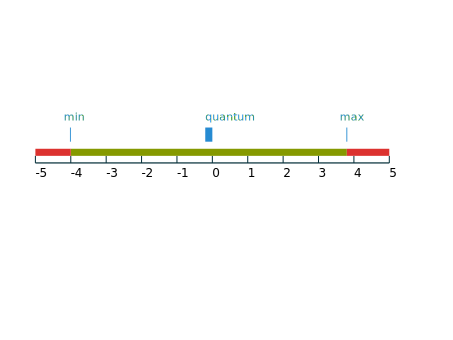
\includegraphics[width=\textwidth]{./src/img/fixedPoint.pdf}
\end{figureGraphics}

The test suite computes some values within the green(valid) area and the
red(invalid) area and performs the checks illustrated on figure \ref{fig:fixedPointTest} below.

\begin{figureGraphics}{Fixed point test suite}{fig:fixedPointTest}
    \includegraphics[height=0.6\textheight]{./src/img/fixedPointProcess.pdf}
\end{figureGraphics}

Below is a small description of the tests:
\begin{description}
    \item[Bound check] The \gls{pfw} should throw an error if we
        attempt to set an out-of-bound value.
    \item[Sanity check] If we manage to set the value, The \gls{pfw} should not modify too much
        the value. It can change by half a quantum at maximum.
    \item[Consistency check] The \gls{pfw} should accept the value it sent previously.
    \item[Bijectivity check] The \gls{pfw} should return the same value we provided it at the Consistency check.
\end{description}

\subsubsection{Rework the internal mechanism}
It was time to rework the internal
mechanism of the \gls{pfw}.

The \gls{pfw} can export parameters to a file. Fixed
point parameters can be exported as well.
\begin{itemize}
    \item When exporting them, the \gls{pfw} converts the value from
        its internal representation towards a floating point number, because that is
        easier to read.
    \item By converting that number, it also computes the amount of digits
        to use for display, or writing towards a file. This can result in
        \emph{rounding issues}, due to limitation of the \lstinline{setPrecision} \gls{cpp} method.
        TODO detail what were the issues (rounding to upper value, etc)
\end{itemize}
The fix I proposed was to replace the computation of displayable digits by something
easier, which is the \emph{Fractional part} of the fixed point number.

The example in listing \ref {lst:fixedPointProblem} illustrates a bound error check, and the output in the corrected version.

\begin{code}[language=bash, caption=$Q.2.3$ rounding issue example, label=lst:fixedPointProblem]
#  broken version  #
####################
$ pfw setParameter /Example/fixedPoint/q2.3 3.875
# Done
$ pfw getParameter /Example/fixedPoint/q2.3
# 3.9 <= this is not expected, since 3.875 is encodable!
$ pfw setParameter /Example/fixedPoint/q2.3 3.9
# Value 3.9 standing out of admitted real range
# [-4, 3.875] for FixedPointParameter /Test/test/q2.3
# ^ this is even weirder

#  fixed version  #
###################
$ pfw setParameter /Example/fixedPoint/q2.3 3.875
# Done
$ pfw getParameter /Example/fixedPoint/q2.3
# 3.875
\end{code}


% {{{2
\subsection{Multiple modem support}
With the \emph{bring your own device} trends, more and more smartphones support dual simcards. This case
is useful to use the same device for corporate and private purposes.
Besided, in some developing countries phone carriers do not cover the whole country. The habitants of those
countries need several phone carriers to use their smartphone smoothly.
For those purposes, the platform must support two modems.
Within the Intel Audio \gls{hal}, we are handling some voice processing algorithms from the signal coming from the modem.
Naturally, we have a \gls{pfw} plugin to abstract the modem. This plugin did not support multiple modems.

I had to add \emph{modem instance awareness} to the plugin. With the current implementation, it
is possible to have multiple structure files, each describing a modem. This would theoretically allow
to support as many modems as we want.

TODO explain a bit more.

% {{{1
\section{Open-sourcing on GitHub}
In order to stimulate the usage of the \gls{pfw} for other projects than the Intel Audio \gls{hal},
our team decided to release the source-code on \gls{GitHub}.
This should favor external contributions via \gls{pullrequests} and motivate
the community to use the \gls{pfw}.

Around this activity, I covered several topics:
\begin{description}
    \item[Communicating, Documentating] the \gls{pfw} components.
    \item[Push, clean, enchance] the code to make sure no proprietary
        elements are made public.
\end{description}

% {{{2
\subsection{Parameter-framework newcomer's documentation}\label{sec:tutorials}

At the start of my internship, I had to inspect the \gls{pfw}'s
source code without any documentation. The idea was to have a fresh look at
this piece of software to determine if it was open-source ready, straightforward
to use, for someone who is unfamiliar with it.

While doing that, I struggled a bit with the basic usage of the framework. The
team decided that it would be nice to have some newcomer tutorials and examples,
for an easier adoption of the open-source community. So I wrote several
tutorials:
\begin{description}
    \item[Compile and install]
        is a step-by-step guide about how to get the \gls{pfw}'s sources,
        build it and install it as a standalone on Ubuntu.
    \item[Run a simple example]
        is a how-to about running the \gls{pfw} command-line interface,
        such as \lstinline{remote-process} and \lstinline {test-platform}.  In
        this how-to, the configuration and setting files are provided so that
        the user can focus on the results. The example covers music play-list
        changing based on a user's mood.
    \item[An introduction to the .pfw language]\label{desc:pfw-language}
        is a tutorial about the .pfw language. This language was
        created to simplify the writing of settings files for the
        \gls{pfw}. Those files are then converted into \gls{xml}, which is
        the only language the \gls{pfw} understands.
\end{description}
These tutorials have been written in \gls{markdown}, the standard format used
on \gls{GitHub}.

% {{{2
\subsection{Parameter-framework's intellectual property}
Intellectual property is very important at Intel. The \gls{pfw} is released under
BSD license. All the source files must contain the correct BSD license header according
to Intel's open-source policy.

\subsubsection{license checker}
Since there are 279 source files released currently on \gls{GitHub}, it seems a lot of
work to check all those files manually.
I wrote an internal tool in \gls{python} which performs the license check semi-automatically.
The script usage is quite straightforward and showed in listing \ref{code:license}.

\begin{code}[language=bash, caption=License checker usage, label=code:license]
usage: license_updater.py [-h] [--cpp | --mk] license root_location

Scans recursively trough directories to find source code which should be
updated with a new license header.

positional arguments:
    license        the license type: ['gpl', 'bsd', 'private']
    root_location  the directory to start scanning

optional arguments:
    -h, --help     show this help message and exit
    --cpp          (default) scan for C++ files: ('h', 'c', 'hpp', 'cpp')
    --mk           scan for Android make files: .mk
\end{code}


% {{{2
\subsection{Branch sync process}\label{sec:syncProcess}
Since we work internally on the \gls{pfw} and can receive external contributions via \gls{pullrequests},
it is quite difficult to keep both repositories in sync.
On figure \ref{fig:branch-process} we can see how we plan to synchronize the different code.

\begin{figureGraphics}{Final branch process}{fig:branch-process}
    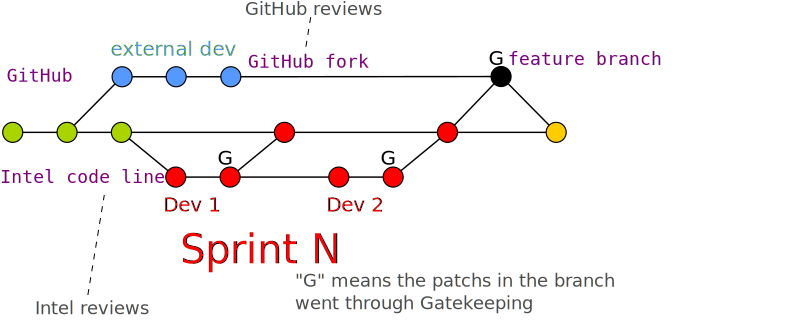
\includegraphics[width=\textwidth]{./src/img/branches-process.pdf}
\end{figureGraphics}


% {{{2
\subsection{Alsa plugin refactoring}
The Alsa plugin is used to handle \gls{alsa} (for desktop mostly) or TinyAlsa (for embedded \gls{android} devices mostly) subsystems.
For our internal uses, we patched some \gls{aosp} projects such as TinyAlsa which allows us to support proprietary controls.
The support of such controls was also implemented in the \gls{alsa} \gls{pfw} plugin. Since
we want to open-source the plugin, those proprietary features should be removed.

During the removal of those special controls, we also simplified the plugin
architecture by merging the controls and the mixer code. TODO removing templates.
The result is a far simpler design.
TODO detail.

% {{{2
\subsection{Code alignment}

When I had to update the different components on \gls{GitHub}, there were some issues:
Our internal version and the \gls{GitHub} one had diverged.
On figure \ref{fig:diverged}, we can see an overview of the branch state before I reworked them.

\begin{figureGraphics}{Repository divergence}{fig:diverged}
    \includegraphics[width=\textwidth]{./src/img/branch-divergence.pdf}
\end{figureGraphics}
Since all the components I uploaded on \gls{GitHub} had modifications which weren't present
in the internal source tree, I encountered the divergence issue for each project I
synchronized with \gls{GitHub} (Core, Alsa and Filesystem).

This was a very good exercise to improve my \gls{git} skill.

\subsection{Core upload}
The \gls{pfw} core is quite a big project, with about 30 000 lines of code.
Align the internal tree and the \gls{GitHub} version of this project required quite some work.
Some extra requirements apply on open-source projects, such as being compilable in a vanilla \gls{aosp} environment.

There is a \gls{GitHub} organization which groups all Intel open-source projects. This
organization is called \emph{01org}. I joined it during my internship in order to have admin rights
on the projects I had to open-source.

The \gls{pfw} core is available on \gls{GitHub}\footnote{\url{https://github.com/01org/parameter-framework}}

% {{{2
\subsection{Filesystem plugin upload}

The file system plugin is used for global access to the filesystem. This can be to
use \emph{/proc} entries for instance. I used this plugin as example in the rookie
documentation I wrote as described in section \ref{sec:tutorials}.

I also worked on an other example: \emph{controlling lEDS} via the filesystem
plugin on a Raspberry Pi.  This example was easy enough to be integrated into
the online documentation of the filesystem plugin, on \gls{GitHub}.

The filesystem plugin is available on \gls{GitHub}\footnote{\url{https://github.com/01org/parameter-framework-plugins-filesystem/}}

% {{{2
\subsection{Alsa plugin upload}

The \gls{alsa} \gls{pfw} plugin is used on within the Intel Audio \gls{hal}. It can also by used
on a linux desktop environement to handle \gls{alsa} mixers.

To demonstrate the power of this plugin, I wrote the README file which is on the
front page on this \gls{GitHub} project.  The README contains :
\begin{itemize}
    \item Build and install instructions
    \item Prerequisites for using this plugin
    \item A tutorial which details how to write the \gls{xml} files for this
    plugin in order to be able to change the master volume on a linux desktop.
\end{itemize}
I also reorganised some code within this plugin since we used to rely on proprietary \gls{aosp} modifications.
This plugin is now vanilla \gls{aosp} compatible, and can be used if the \gls{pfw} is installed.

The \gls{alsa} plugin is available on \gls{GitHub}\footnote{\url{https://github.com/01org/parameter-framework-plugins-alsa/}}
 % WHAT I CREATED at work
\chapter{Conclusion}
\section{subsect}
\subsection{subsub}
Hello, world.
Lorem ipsum dolar

AAAA bscdde

\subsection{}

\section{Global conclusion}
 % WHAT I have learned

%\bibliography{./src/biblio}
%\chapter{Annexes}

\section{Table des annexes}
\begin{description}
  \item[Opérations implémentées] Figure \ref{fig:opImpl} sur la page \pageref{fig:opImpl}
  \item[constants.vhd] Listing \ref{src:constants} sur la page \pageref{src:constants} 
  \item[cpu\_package.2.vhd] \ref{src:cpupackage} sur la page \pageref{src:cpupackage} 
  \item[memory.1.vhd] \ref{src:memory} sur la page \pageref{src:memory}
  \item[pipelineRegisters.vhd] \ref{src:pipelineReg} sur la page \pageref{src:pipelineReg}
  \item[registres.1.vhd] \ref{src:regs} sur la page \pageref{src:regs}
  \item[risc.0.vhd] \ref{src:risc} sur la page \pageref{src:risc}
\end{description}

\section{Liste des instructions implémentées}
      \begin{figureGraphics}{Liste des instructions implémentées}{fig:opImpl}
        \centering
        \begin{tabular}{|l|l|r|}
          \hline
          Catégorie  &  Instruction &  Implémenté \\
          \hline
          \hline
          Arithmétique  &  add  &  oui\\
          \hline
                         &  sub  &  oui\\
          \hline
                         &  addi  &  oui\\
          \hline
                         &  addu  &  oui\\
          \hline
                         &  subu  &  oui\\
          \hline
                         &  addiu  &  oui\\
          \hline
                Logique  &  and  &  oui\\
          \hline
                         &  or  &  oui\\
          \hline
                         &  xor  &  oui\\
          \hline
                         &  nor  &  oui\\
          \hline
                         &  andi  &  oui\\
          \hline
                         &  ori  &  oui \\ 
          \hline
                         &  xori  &  oui\\
          \hline
                         &  lsl  &  oui\\
          \hline
                         &  lsr  &  oui\\
          \hline
          \hline
             Chart. imm  &  lui  &  oui\\
          \hline
              Transfert  &  lb  &  oui\\
          \hline
                     de  &  lh  &  oui\\
          \hline
               données  &  lw  &  oui\\
          \hline
                         &  lbu  &  oui\\
          \hline
                         &  lhu  &  oui\\
          \hline
                         &  sb  &  oui\\
          \hline
                         &  sh  &  oui\\
          \hline
                         &  sw  &  oui\\
          \hline
          \hline
            Branchement  &  beq  &  oui\\
          \hline
           conditionnel  &  bne  &  oui\\
          \hline
                         &  bltz  &  oui\\
          \hline
                         &  blez  &  oui\\
          \hline
                         &  bgtz  &  oui\\
          \hline
                         &  bgez  &  oui\\
          \hline
                         &  bltzal  &  non\\
          \hline
                         &  bgezal  &  non\\
          \hline
                         &  slt  &  non\\
          \hline
                         &  sltu  &  non\\
          \hline
                         &  sltu  &  non\\
          \hline
                         &  sltiu  &  non\\
          \hline
          \hline
                   Saut  &  j  &  oui\\
          \hline
         Inconditionnel  &  jr  &  oui\\
          \hline
                         &  jal  &  oui\\
          \hline
                         &  jalr  &  oui\\
          \hline
        \end{tabular}
      \end{figureGraphics}

\section{Sources VHDL}

%change geom for source listing
\newgeometry{left=2.5cm,right=2.5cm}

\lstinputlisting[language=VHDL, caption=constants.vhd, label=src:constants]{../src/constants.vhd}
\lstinputlisting[language=VHDL, caption=cpu\_package.2.vhd, label=src:cpupackage]{../src/cpu_package.2.vhd}
\lstinputlisting[language=VHDL, caption=memory.1.vhd, label=src:memory]{../src/memory.1.vhd}
\lstinputlisting[language=VHDL, caption=pipelineRegisters.vhd, label=src:pipelineReg]{../src/pipelineRegisters.vhd}
\lstinputlisting[language=VHDL, caption=registres.1.vhd, label=src:regs]{../src/registres.1.vhd}
\lstinputlisting[language=VHDL, caption=risc.0.vhd, label=src:risc]{../src/risc.0.vhd}

\end{document}
